\documentclass[3p,twocolumn]{elsarticle}
%%\usepackage[utf8]{inputenc}
%%\usepackage[LGR,T1]{fontenc}
%%\usepackage{graphicx,amsmath}
%%\usepackage[british]{babel}
%%\usepackage[latin9]{inputenc}%SOME KIND OF CLASH WITH THIS ONE
%%\usepackage{array}
%%\usepackage{rotfloat}
%%\usepackage{textcomp}
%%\usepackage{amssymb}
%%\usepackage{amsmath} % to align equations \usepackage{mathrsfs} % curly font in math, called using mathscr
%%\usepackage{graphicx}
%%\usepackage{subcaption} % to have two images under one caption
%%\usepackage{subscript}
%%\usepackage{gensymb} %for degree symbol
\setlength{\marginparwidth}{2cm} % to set the width of the marginpar
\usepackage{todonotes}
%%\usepackage{xargs}                      % Use more than one optional parameter in a new commands
%%\renewcommand{\baselinestretch}{1.5}
\bibliographystyle{elsarticle-num}
\begin{document}
\begin{frontmatter}
\title{Advanced Characterisation of Pore Structure in Next-Generation Reactor Graphites}
\author[plym]{Bradley Moresby-White}
\author[plym]{Katie L. Jones\corref{cor1}}
\ead{katie.jones@plymouth.ac.uk}
\author[plym]{G. Peter Matthews}
\author[plym]{Giuliano M. Laudone}
\cortext[cor1]{Corresponding author.}
\address[plym]{Faculty of Science and Engineering, University of Plymouth, Plymouth, UK}
\begin{abstract}
Nuclear grade graphite
\end{abstract}
\begin{keyword}keyword\sep keyword\sep keyword\end{keyword}
\end{frontmatter}

\section{Introduction}
This is a citation.\cite{JONES2020256HgHe}

\section{Methodology}

\subsection{Materials}

Virgin graphite samples of two grades, IG‑110 and IG‑430, were supplied by
Toyo Tanso Ltd\texttrademark, Osaka, Japan. The properties of both grades are tabulated (Table
~\ref{tab:materialstable}).

\begin{table*}[t]
  \centering
  \caption{Manufacturer's characterisation of the graphite types \citep{Jones2018}}
  \label{tab:materialstable}
  \resizebox{\textwidth}{!}{%
    \begin{tabular}{l l c c c c c}
      \hline
      Grade   & Coke source & Bulk density/g cm$^3$ & Filler particle size/$\mu$m) & Tensile strength/MPa & Young's modulus/GPa & Thermal conductivity/W m$^{-1}$K$^{-1}$\\
      \hline
      IG‑110  & Petrol            & 1.77                  & 10                           & 25                     & 9.8                   & 120 \\
      IG‑430  & Pitch             & 1.82                  & 10                           & 37                     & 10.8                  & 140 \\
      \hline
    \end{tabular}%
  }
\end{table*}

IG‑110 is currently employed in the three existing HTGRs worldwide, while IG‑430 is
designed to deliver increased density, strength, and thermal conductivity for future
applications.\citep{toyotanso_atomic_nuclear} (Table ~\ref{tab:materialstable}).
Both grades comply with \textit{ASTMD7219-19}, including the requirement for
a minimum bulk density exceeding 1.7 g/cm$^3$ \citep{ASTMD7219-19} 
(Table~\ref{tab:materialstable}).

\subsection{Sample preparation}

The cuboids were sub-sampled from the virgin graphite blocks, with dimensions of
approximately 10 mm x 10 mm x 100 mm. The sub-samples were further subsampled into
cuobids of side lengths ~7mm, providing 3 cuboids per grade. Samples were polished
via SiC polishing pads up to a grit size of P5000, to minimise topographical variations
induced by sample preparation  that could scatter the electron beam during SEM, potentially
 causing artifacts \citep{Fang2022}.Samples were sonicated in 2-propanol for 24h to
remove any contaminants introduced by the lubricant used in the machining process.
 The samples were then dried under vacuum for 12 h at $305 \pm 5\,^\circ\mathrm{C}$ using
the BELPREP-vac (MicrotracBEL, Japan) in order to remove any residual moisture introduced
during the sonication process.

\subsection{Micrograph generation}
The JEOL\texttrademark IT510 Scanning Electron Microscope was used in the
generation of the contiguous set of individual micrographs from which the full
composite is assembled. The \textit{Image Montage} capability, within the
JEOLInScope\texttrademark package, performed this function. The system captures 
a set number of micrographs, with the motorised stage moving the electron beam over
the specified area with a set overlap, with the software adjusting stigmation, contrast,
and brightness. Shifts in contrast and brightness were on the order of 1\% \todo{Make sure to double check that figure for ACB} and thus negligible in affecting the final
thresholded image, particularly following fusion. The parameters selected are
tabulated (Table ~\ref{tab:microscopy_parameters}).

\subsection{Composite assembly}

The composite assembly (i.e., "stitching") stage has a significant impact on
the porosity values derived from the final composite, as incorrect fusion will
misrepresent pore structures. A stitching method based on the phase correlation
approach originally developed by \citet{Kuglin1975}, amongst the most popular
and well-tested approaches available for image registration, was selected and
operated as a plug-in within ImageJ/Fiji \citep{Preibisch2009}. This method
represents a development of the original phase correlation method, and was
selected for its solid mathematical foundations\citep{Preibisch2009}.
	
	The mathematics of phase correlation methods is further detailed in the
	Appendix. In this work, the primary advantage is the application of a
	smooth, non-linear intensity transition between the overlapping micrographs.
	This is a prerequisite as the selection of an intensity threshold is not
	possible if the variations in contrast and brightness between micrographs
	are non-trivial. Additionally, this method also avoids the propagation of
	errors by consecutive registration steps, which is key at this scale
	\citep{Preibisch2009}. Another benefit is the sub-pixel accuracy of the
	fusion, as incorrect alignments would generate false pore diameters.
	Finally, the method is computationally efficient, which is important where
	the input micrographs sum to several hundred megabytes in size.



\begin{table*}[ht]
  \centering
  \caption{Parameters for composite assembly captured with the JEOL IT510 SEM using Image Montage Mode}
  \label{tab:microscopy_parameters}
  \resizebox{\textwidth}{!}{%
    \begin{tabular}{l l}
      \hline
      Parameters & Values \\
      \hline
      Magnification (X)                    & 1000 \\
      Resolution ($\mu$m/px)               & 0.1 \\
      Surface area per micrograph ($\mu$m$^2$) & 12\,288 \\
      Overlap (\%)                          & 10 \\
      Micrographs per sample (n)            & 196 \\
      \hline
    \end{tabular}%
  }
\end{table*}

\begin{figure}[ht]
    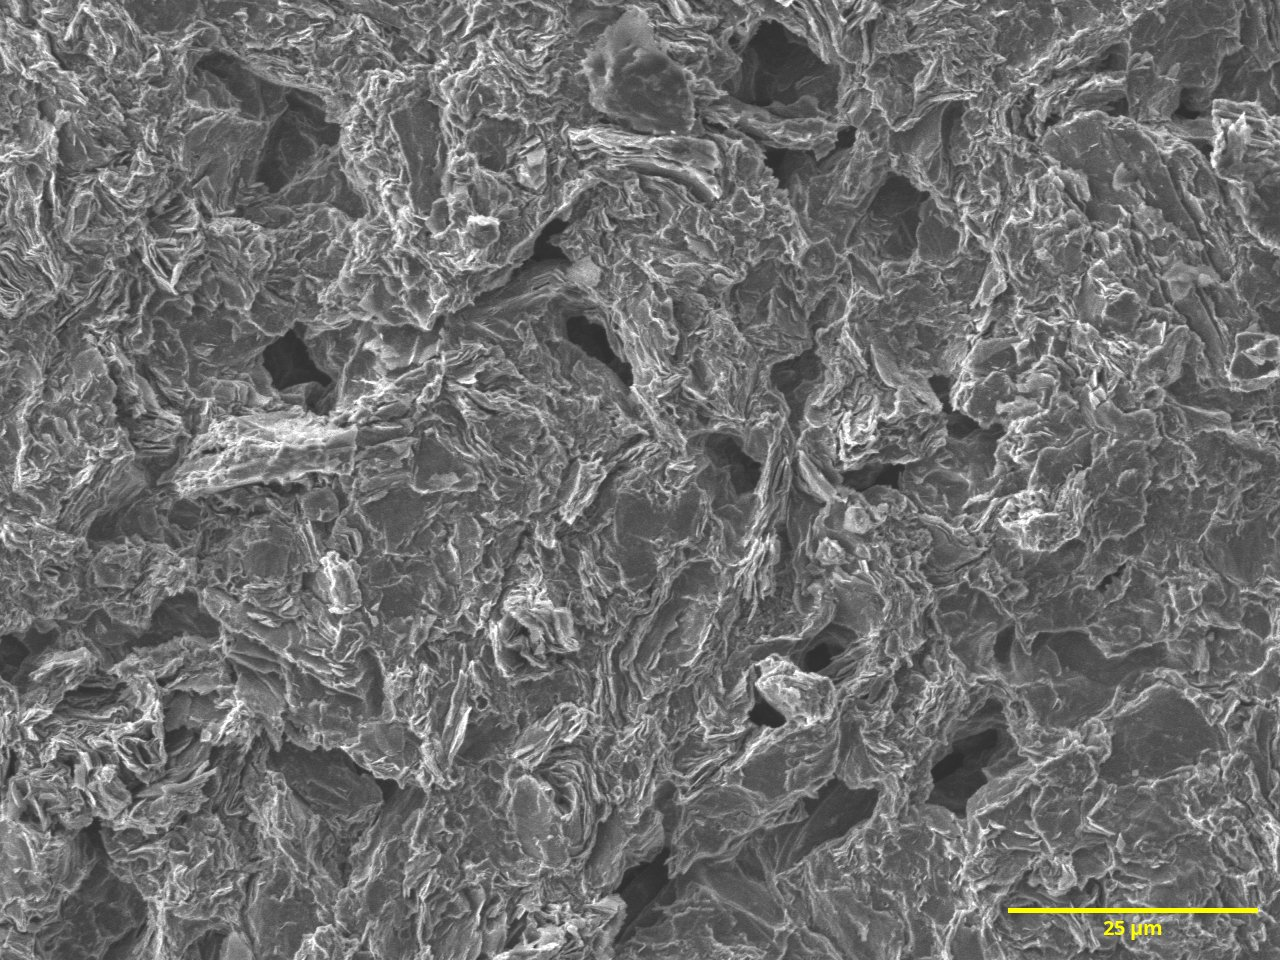
\includegraphics[width=0.45\textwidth]{./Media/image.png}
    \caption{PLACEHOLDER}
    \label{fig:testimage1}
\end{figure}
\clearpage
\bibliography{bibliography}
\end{document}